\section{Results}
\subsection{Survey results in summary}
\justify

%- Present results in the order of the research questions
%- (Amount of records, amount of faulty records)
%- Uncertainties
%- Present logically all results and interesting specific questions
%- Compare parking with original Travel Time Matrix values and values collected by me
%- Charts, statistics
%- Just show your findings, no nonsense
In this chapter we will discuss the thesis research survey results which fit the criteria discussed in \hyperref[sec:processdata]{\fullref{sec:processdata}}. Within the selected criteria, the survey received a total of 5579 visits from 4320 unique IP addresses. 848 unique IP addresses visited the survey more than one time and in total 1060 unique IP addresses sent data to the survey. 24.5 percent of all visitors submitted at least one data row. On average one respondent submitted 4.9 data rows.

The survey received in total 5183 data rows. All postal code areas were represented in the survey results (figure~\ref{fig:postalvis_answers}), but the data row count histogram was heavily skewed to the right, with the first quartile being eight data rows, second (median) 17 data rows and third 42 data rows (table~\ref{tab:muns_answer_stats}). There were five postal code areas with more than one hundred data rows and 55 postal code areas with less than ten data rows. In Helsinki the answers strongly clustered around the center of Helsinki, with other centers of activity being Herttoniemi and Itäkeskus-Marjaniemi in Helsinki, Tapiola-Otaniemi and Leppävaara in Espoo, and Tikkurila-Vantaanportti in Vantaa.

On a closer look to the municipalities finer details become apparent. For example, in Helsinki a wedge-like area of survey activity in the direction of southwest-northeast is visible. Starting out from the west, this area spans from Lauttasaari to the center of Helsinki and moving on all the way to Malmi. Many of the areas around the research area which could be roughly characterised as residential areas were left with little activity. Furthermore, in the survey instructions respondents were requested to refrain from including parking activity in private property, as it was assumed that these areas would provide near to instantaneous parking. The lightness of activity in residential areas corresponds with the made request.

\begin{hyphenrules}{nohyphenation}
    \begin{table}[H]
        \centering
        \def\arraystretch{1.2}
        \setlength\tabcolsep{4pt}
        \caption[Answer counts by municipality]{Amount of data rows received per municipality in Helsinki Capital Region.} 
        \label{tab:muns_answer_stats}
        \begin{tabular}{ @{} >{\raggedright\arraybackslash}p{3cm} >{\raggedright\arraybackslash}p{2cm} >{\raggedright\arraybackslash}p{4cm} >{\raggedright\arraybackslash}p{2cm} >{\raggedright\arraybackslash}p{2cm} @{} }
            \toprule
            Municipality & Data rows total & Most data rows in municipality & Mean & Median \\
            \midrule
            Helsinki & 3777 & 271 (00100 Helsinki Keskusta - Etu-Töölö) & 45.0 & 34.5 \\
            Espoo & 637 & 84 (02600 Etelä-Leppävaara) & 17.7 & 9 \\
            Vantaa & 746 & 91 (01510 Kirkonkylä-Veromäki) & 16.2 & 8 \\
            Kauniainen & 23 & 23 (02700 Kauniainen) & 23 & 23 \\
            % use \usepackage[table]{xcolor} and \usepackage{booktabs} to define \greyrule
            \greyrule
            All & 5183 & 271 (00100 Helsinki Keskusta - Etu-Töölö) & 31.0 & 17 \\
            \bottomrule
        \end{tabular}
    \end{table} 
\end{hyphenrules}

\begin{figure}[H]%
    \centering
    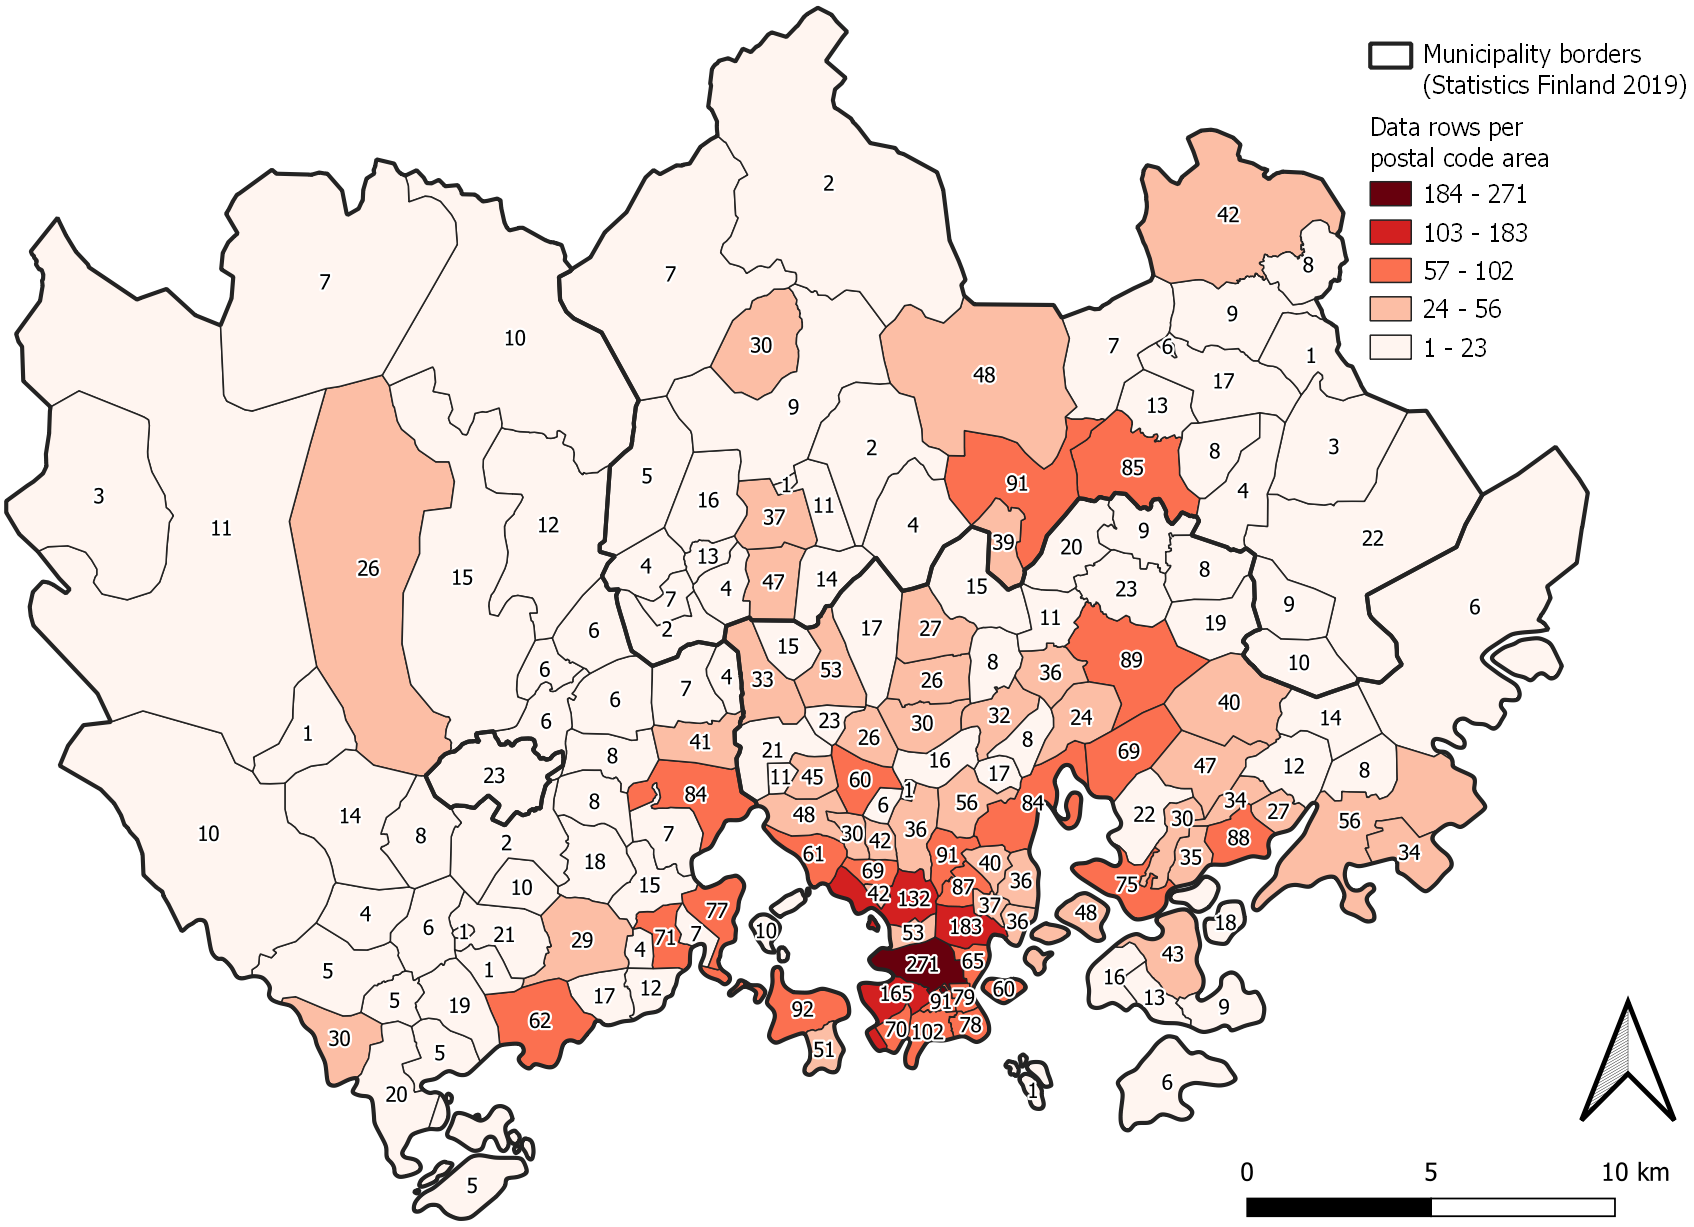
\includegraphics[width=.88\textwidth]{images/thesis_postalvis_answers.png}
    \caption[Data rows received per postal code area]{This figure illustrates the data rows received in the survey per postal code area (n=167). Classes are in natural breaks (Jenks). Municipality borders are based on \textit{postal} data.}%
    \label{fig:postalvis_answers}%
\end{figure}

\begin{figure}[H]%
    \centering
    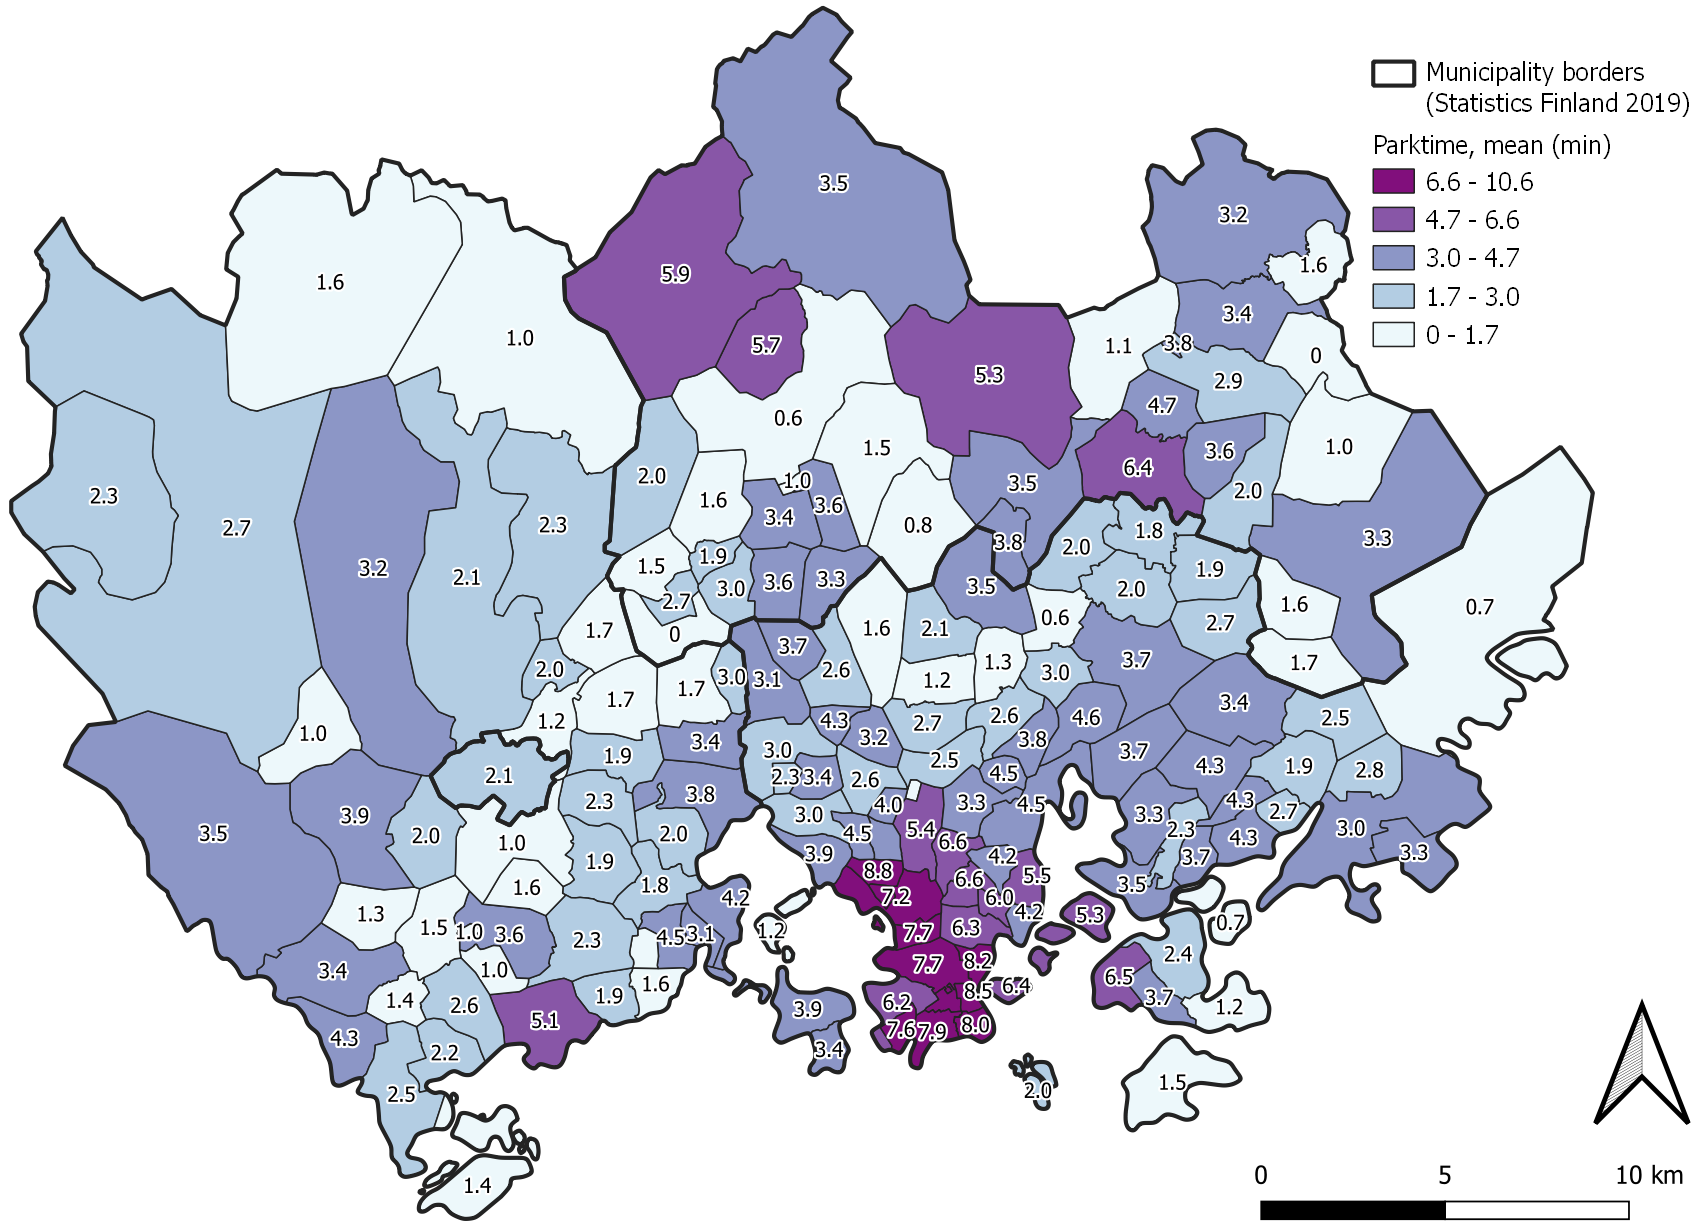
\includegraphics[width=.88\textwidth]{images/thesis_postalvis_parkmean.png}
    \caption[Parktime, mean, in the reseach area]{This figure illustrates the mean duration of searching for parking and parking one's car, usually, in each postal code area.}%
    \label{fig:postalvis_parkmean}%
\end{figure}

\begin{figure}[H]%
    \centering
    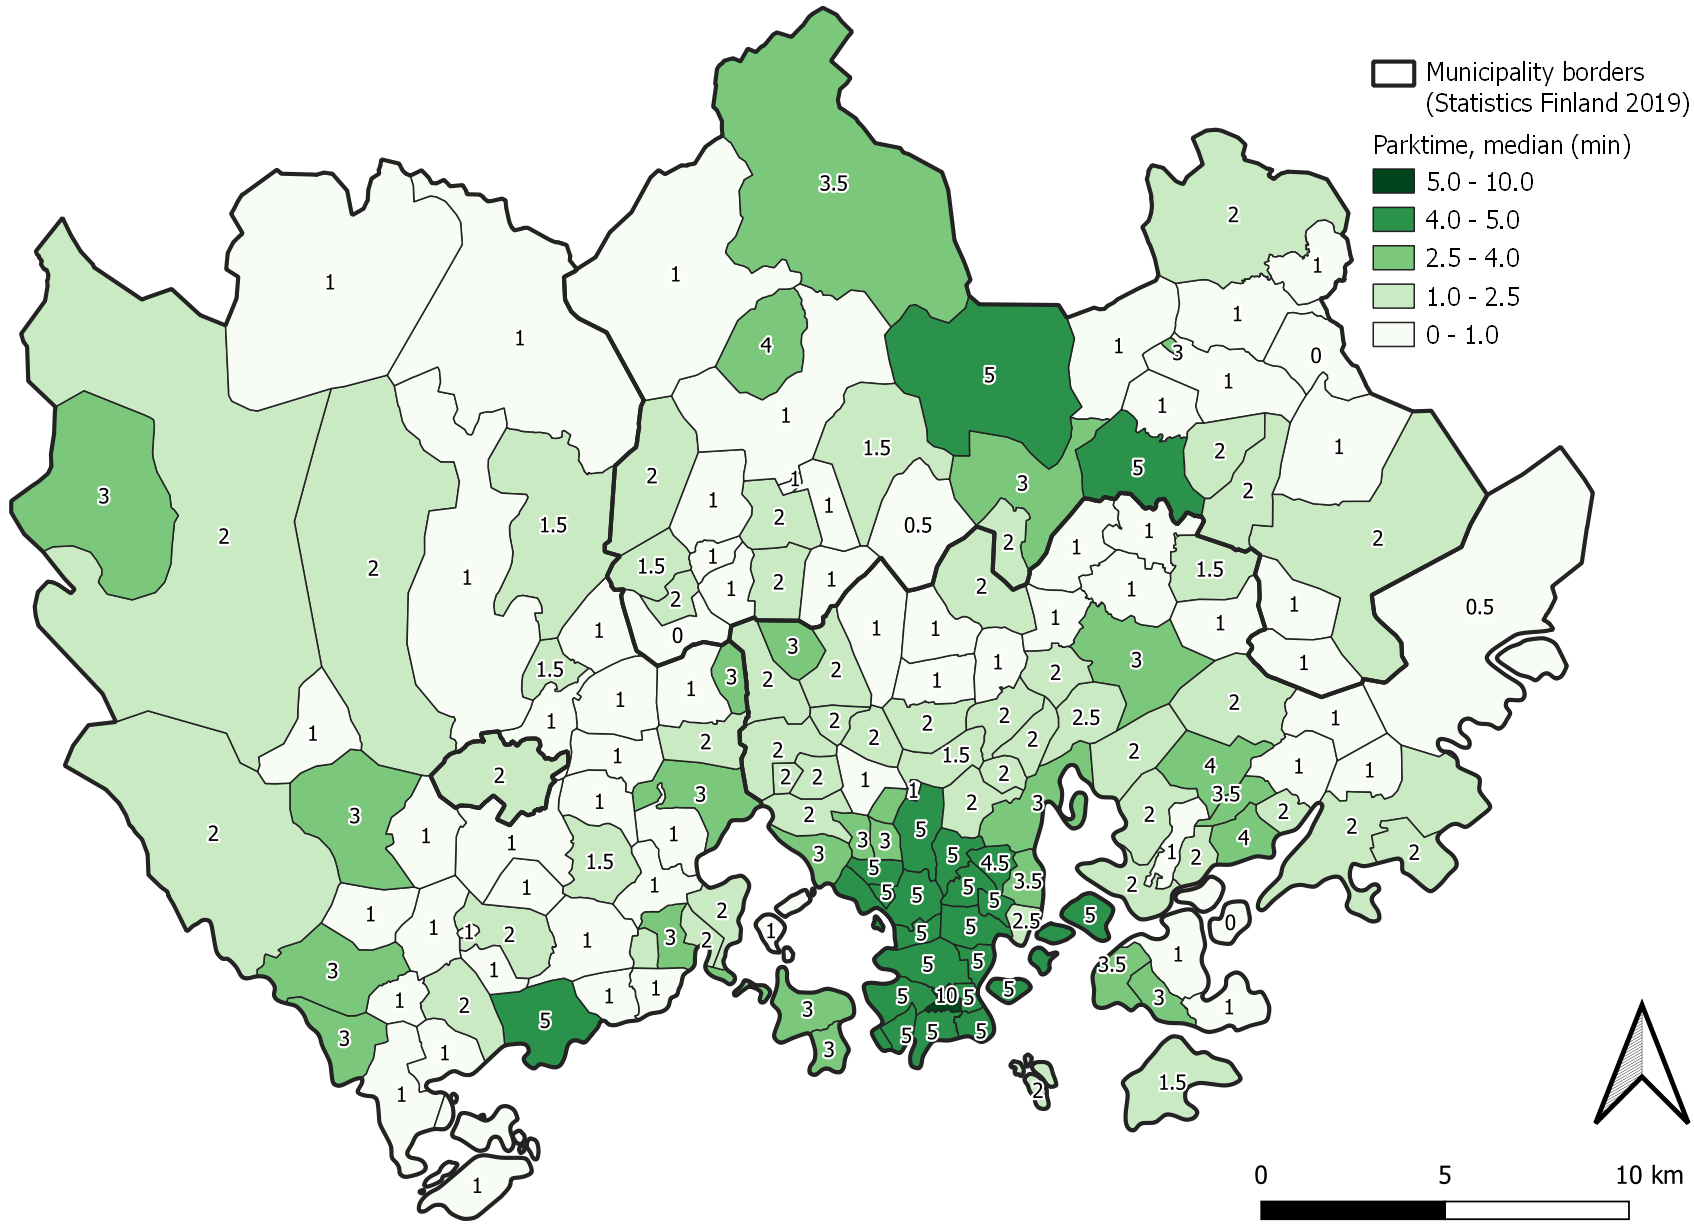
\includegraphics[width=.88\textwidth]{images/thesis_postalvis_parkmedian.png}
    \caption[Parktime, median, in the reseach area]{This figure illustrates the median duration of searching for parking and parking one's car, usually, in each postal code area.}%
    \label{fig:postalvis_parkmedian}%
\end{figure}

\begin{figure}[H]%
    \centering
    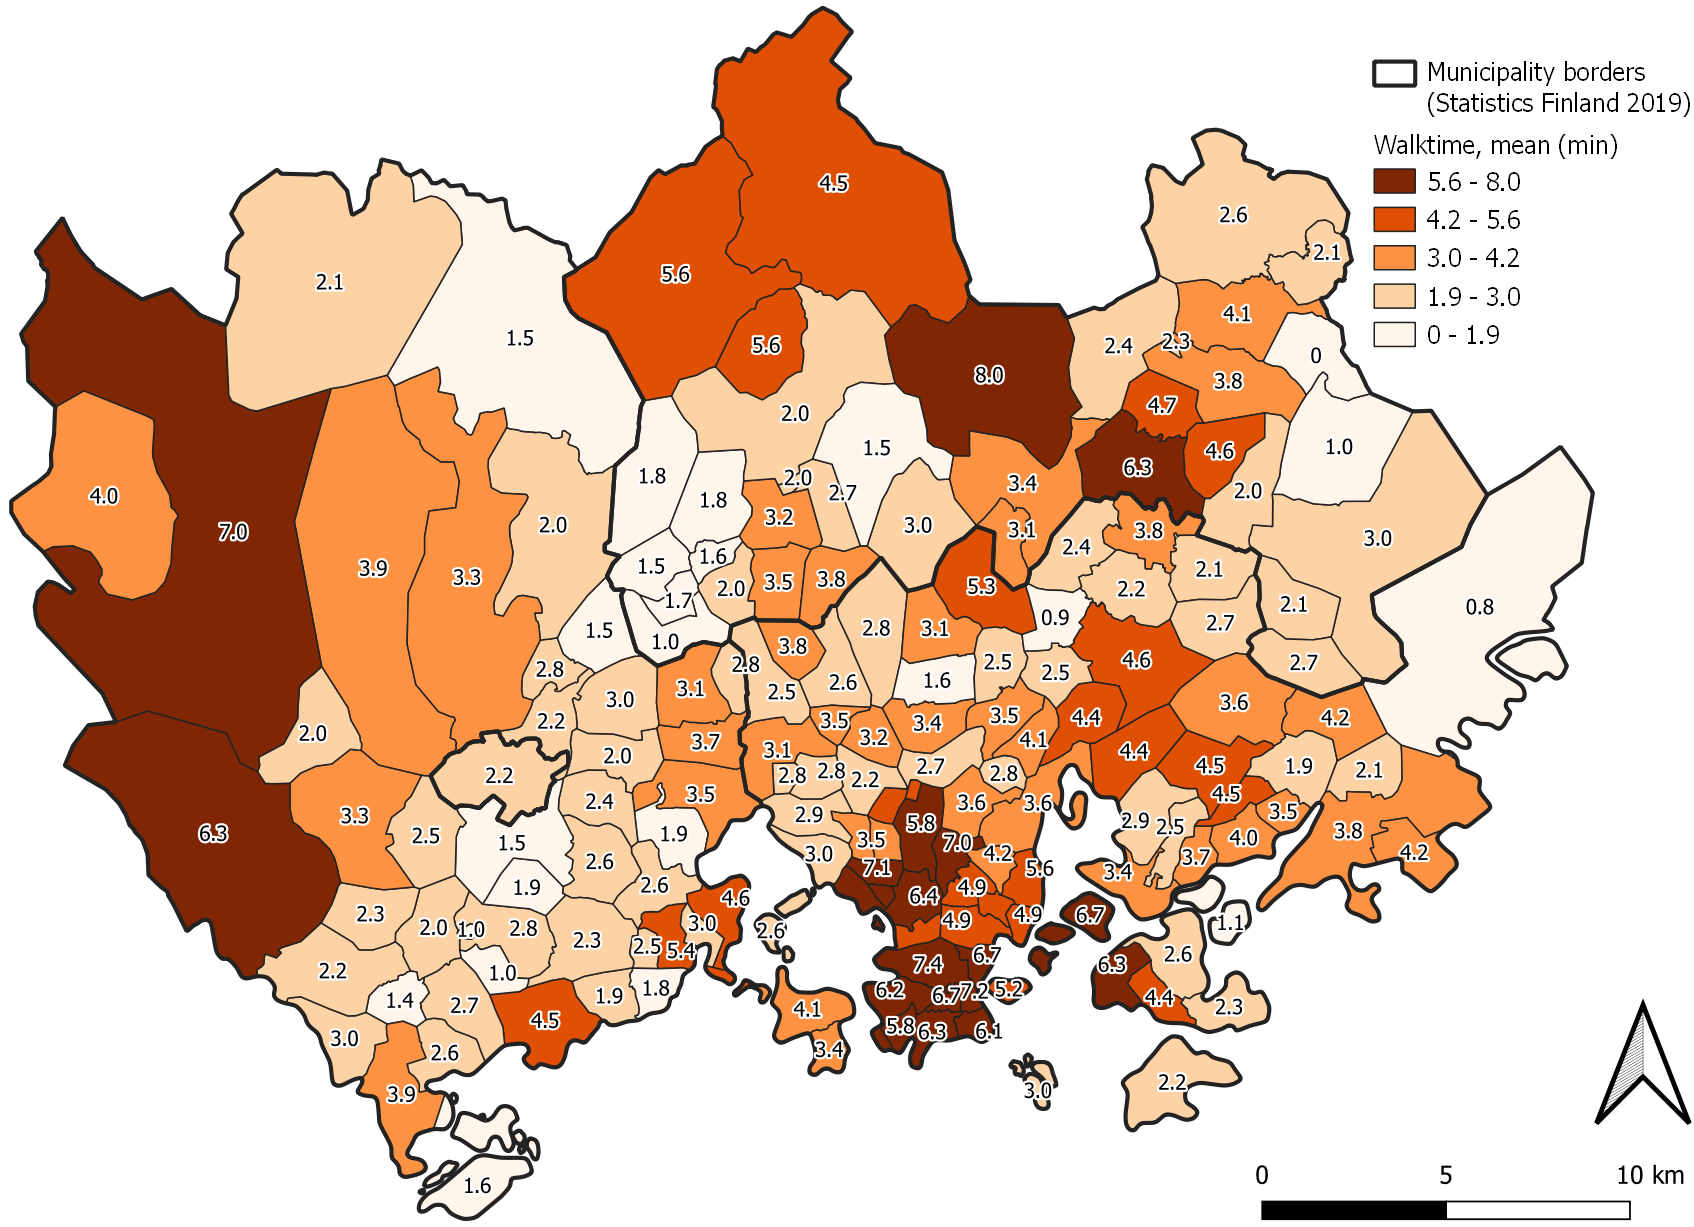
\includegraphics[width=.88\textwidth]{images/thesis_postalvis_walkmean.png}
    \caption[Walktime, mean, in the research area]{This figure illustrates the mean duration of walking from one's parked car to the final destination, usually, in each postal code area.}%
    \label{fig:postalvis_walkmean}%
\end{figure}

\begin{figure}[H]%
    \centering
    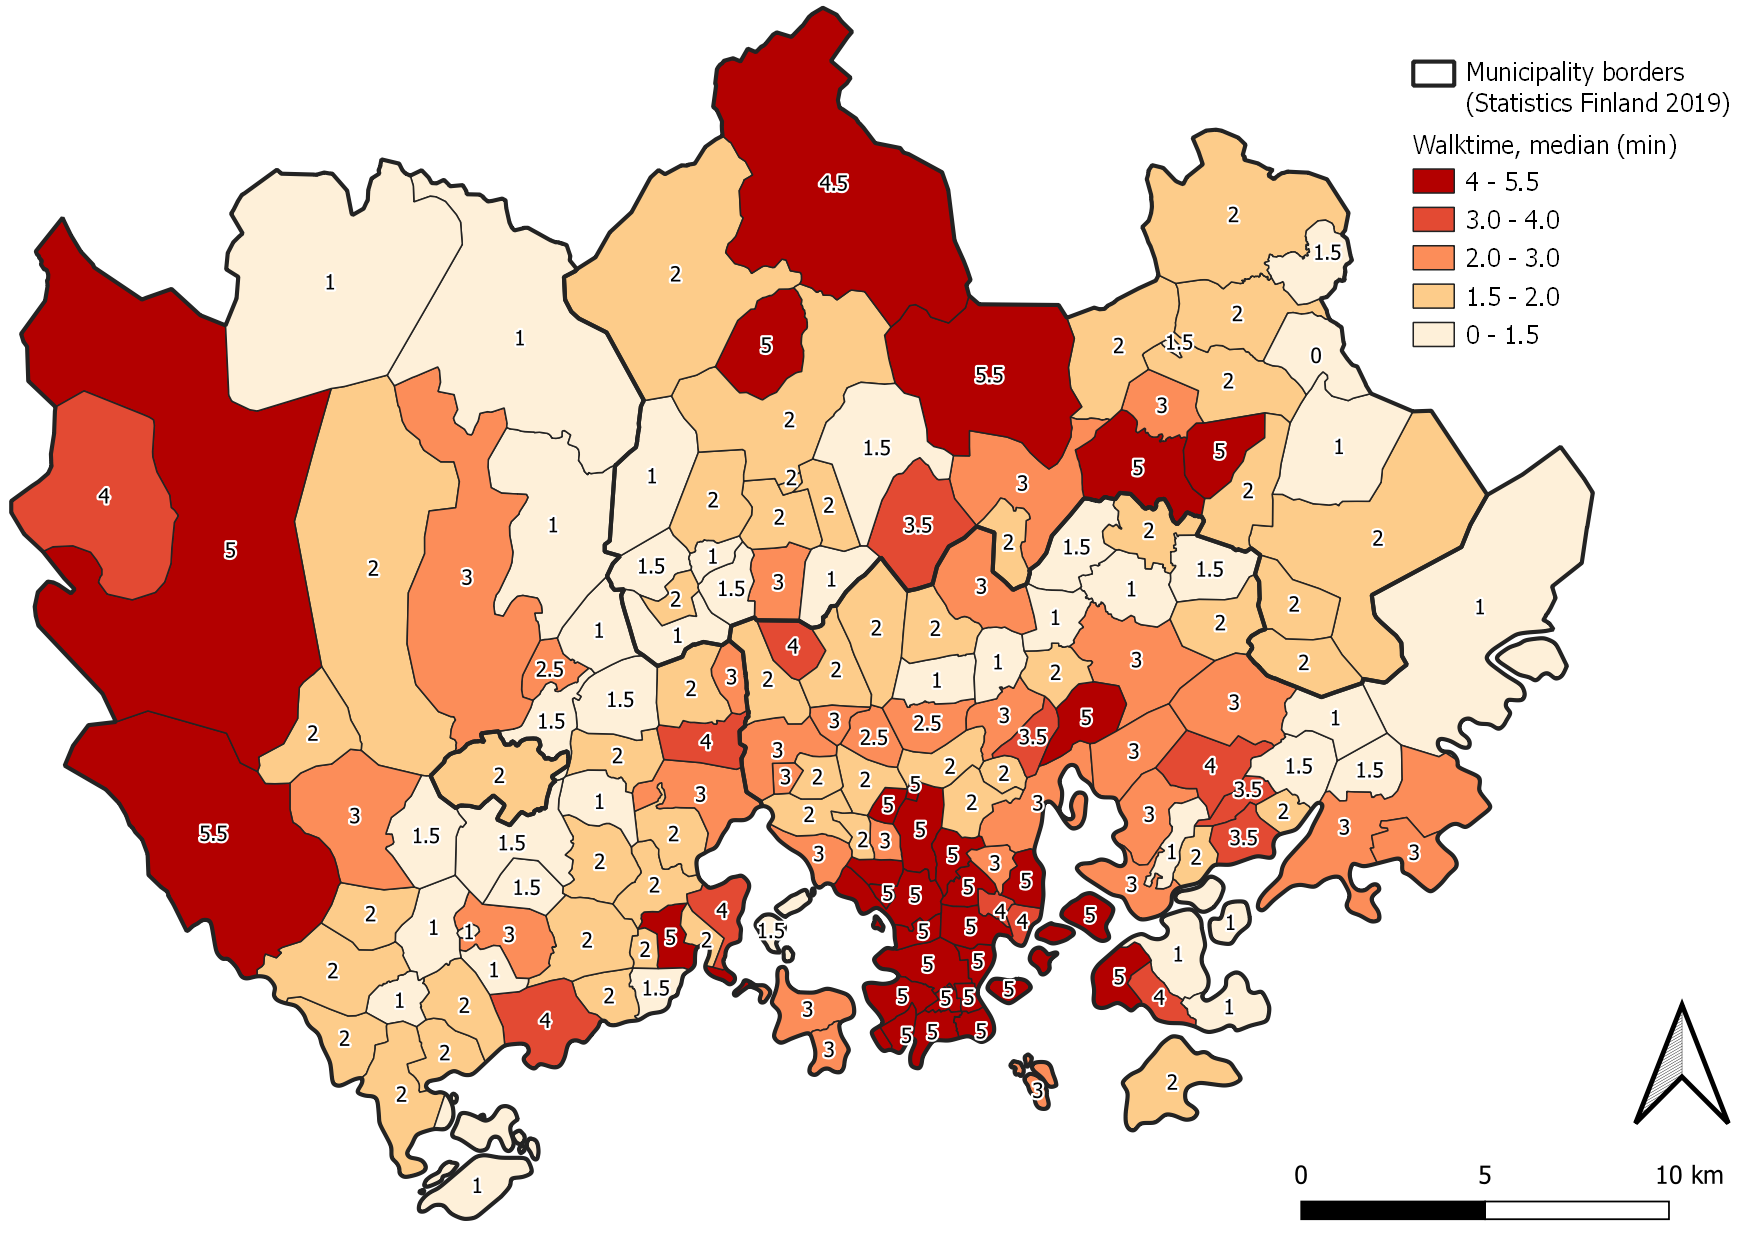
\includegraphics[width=.88\textwidth]{images/thesis_postalvis_walkmedian.png}
    \caption[Walktime, median, in the research area]{This figure illustrates the median duration of walking from one's parked car to the final destination, usually, in each postal code area.}%
    \label{fig:postalvis_walkmedian}%
\end{figure}

\newpage
\subsection{Statistics}
\justify

The survey data shows that there are spatial differences in the parking times and walking times between municipalities and regions of Helsinki Capital Region (table~\ref{tab:parktimes_walktimes}). It is shown by the one-way analysis of variance test (ANOVA) that for parktime and walktime there are statistically significant differences between groups (municipality subdivisions). These differences are wide ranging, with mean parking time in Helsinki being 5.2 minutes, 3.8 minutes in Vantaa, 3.2 minutes in Espoo and lastly, 2.1 minutes in Kauniainen. Parking times vary inside municipalities; in Espoo, in the subdivision of Pohjois-Espoo mean parking time was 1.7 minutes while the same value for Suur-Matinkylä was 4.3 minutes. From all the subdivisions in the research area, the subdivision representing the center of Helsinki, Helsinki Southern, had the the longest mean parking time, 7.3 minutes. In the vast majority of subdivision groups the group sizes were sufficiently large for ANOVA analysis to be significant. This was also true for sample sizes across the board.

In the finest resolution available, the postal code areas, the parking times closely follow those described in the subdivision scale. The longest mean parking times are encountered in the center of Helsinki, where the value for Punavuori is 10.6 minutes (91 data rows) and Meilahden sairaala-alue 9.4 minutes (42 data rows). Mean parking times over five minutes are recorded in all over the center area, but also in Kulosaari (5.3 minutes, 48 data rows) and Kaitalahti (6.5 minutes, 16 data rows). In Espoo, the longest mean parking times were found from Matinkylä (5.1 minutes, 62 data rows) and Tapiola (4.6 minutes, 71 data rows) and in Espoonlahti with 4.3 minutes to generally find a parking spot (30 data rows). In Vantaa, the vicinity of Helsinki-Vantaa airport is not as apparent as with subdivisions. It took the longest to find a parking spot in Tikkurila with 6.4 minutes (85 data rows). According to the results it was relatively hard to find a parking spot in Keimola (5.9 minutes, 7 data rows) and Kivistö (5.7 minutes, 30 data rows), too.

The mean walking times follow the same order as parking times: On average, in Helsinki it took 4.8 minutes to walk from one's parked car to the final destination of the journey. In Vantaa this process was 4.0 minutes, while Espoo had mean parking time of 3.9 minutes and Kauniainen 2.2 minutes. Of the entire research area, Espoo's Suur-Kauklahti stood out with a mean walking time of 6.3 minutes to one's destination. It is notable that this subdivision received 10 answers, ranking second to the last after Helsinki's Östersundom's total of 6 answers.

When viewed through postal code areas, walking time shows somewhat different results when compared to the coarser resolution view of municipality subdivisions. In Helsinki, the longest mean walking time to one's destination was 7.39 minutes in Helsinki keskusta -- Etu-Töölö. Most of the central Helsinki did not fall far behind with most values ranging from five minutes to seven minutes. Outside of the center of Helsinki, Kulosaari (6.7 minutes, 48 data rows), Kaitalahti (6.3 minutes, 16 data rows) and Tuomarinkylä-Torpparinmäki (5.3 minutes, 15 data rows) saw long walking times within the boundaries of Helsinki. Conversely, the walking times in Espoo were mostly lower than those in Helsinki. Longest walking times in Espoo were seen in Tapiola (5.4 minutes, 71 data rows), Kauklahti (6.3 minutes, 10 data rows), and Nupuri-Nuuksio (7.0 minutes, 7 data rows). Vantaa's longest mean walking times were found in Veromiehenkylä (8.0 minutes, 48 data rows), Tikkurila (6.3 minutes, 85 data rows), and Kivistö (5.6 minutes, 30 data rows). It is a potential pitfall to try and determine the causes behind these values, but it may be worth noting, that many of the long walktime postal code areas contain popular sightseeing locations, such as the Haltiala domestic animal farm in Tuomarinkylä-Torpparinmäki and the national park of Nuuksio in Nupuri-Nuuksio. The postal code area of Veromiehenkylä is almost entirely in the use of Helsinki-Vantaa airport.

%https://www.researchgate.net/post/Is_there_a_minimum_number_per_group_neccessary_for_an_ANOVA
%anova - ryhmän koko anovassa
% interpret anova table in r
%http://www.understandingdata.net/2017/05/11/anova-tables-in-r/
%https://www.statisticssolutions.com/sample-size-calculation-for-one-way-anovas-in-dissertations-and-theses/

%levene näyttää vain vähän eri, niin ei oo välii, sitten pitäis kattoo keskihajontaa
%anova pitäis olla ok koska 20 tapausta jo riittävä tuloksen löytymiseen 
%voin todeta, että on tilastolliseti merkitsevä ero, sitten vaan raportoi mikä on ero, esim espoo vs helsinki
%anova todistaa, että kaikilla esim "subdiveillä" ei ole samoja arvoja
%-- parittaiset t-testit jos haluaa kahden paikan välillä testailla
%-- viikonloppuaikojen sisällä varianssi ja viikonpäivän varianssi, kuinka paljon varianssista se selittää
%-- power-analyysi?? Eta-squared (eta2)

%https://statistics.laerd.com/spss-tutorials/one-way-anova-using-spss-statistics-2.php
%LINKISTÄ: therefore, there is a statistically significant difference in the
%mean length of time to complete the spreadsheet problem between the different 
%courses taken.

\begin{hyphenrules}{nohyphenation}
    \begin{table}[H]
        \centering
        \caption[Parktime and walktime descriptive statistics]{Parking times and walking times descriptive statistics displayed by municipalities and subdivisions (n=5183). The unit in median and mean is minutes.}
        \label{tab:parktimes_walktimes}
        \scalebox{0.8}
        % Column type C is a custom column which adds space to its position. Used to separate important features of this table. L aligns left.
        {\begin{tabular}{clLcccCccccc}
            \toprule
            & & &                                       \multicolumn{4}{c}{Parktime} &      \multicolumn{4}{c}{Walktime} \\
                                                        \cmidrule(lr{\tbspace}){4-7}        \cmidrule(lr){8-11}
            & & n &                                     Median & Mean & Std.dev & Std.err & Median & Mean & Std.dev & Std.err \\
            \midrule
            \multirow{7}{*}{Espoo} & Pohjois-Espoo &    29 & 1 & 1.69 & 2.12 & 0.39 &    1 & 1.86 & 1.55 & 0.29 \\
            & Suur-Espoonlahti &                        99 & 2 & 2.88 & 3.27 & 0.33 &    2 & 2.83 & 2.67 & 0.27 \\
            & Suur-Kauklahti &                          10 & 2 & 3.50 & 3.69 & 1.17 &    5.5 & 6.30 & 4.81 & 1.52 \\
            & Suur-Leppävaara &                         176 & 2 & 3.12 & 2.94 & 0.22 &   3 & 3.27 & 2.41 & 0.18 \\
            & Suur-Matinkylä &                          95 & 3 & 4.28 & 4.05 & 0.42 &    3 & 3.76 & 2.81 & 0.29 \\
            & Suur-Tapiola &                            257 & 2 & 3.33 & 3.94 & 0.25 &   2 & 3.84 & 3.41 & 0.21 \\
            & Vanha-Espoo &                             80 & 2 & 2.81 & 4.00 & 0.45 &    3 & 3.89 & 3.81 & 0.43 \\
            % Use \arrayrulecolor to get a grey cmidrule, then revert \midrule color back to black
            \arrayrulecolor{black!30}\cmidrule(lr){2-11}
            & \textbf{Total} &                          746 & 2 & 3.23 & 3.63 & 0.13 &   2 & 3.52 & 3.09 & 0.11 \\
            \arrayrulecolor{black}\midrule
            \multirow{8}{*}{Helsinki} & Central &       704 & 5 & 5.54 & 5.72 & 0.22 &   5 & 4.91 & 3.92 & 0.15 \\
            & Eastern &                                 360 & 2 & 3.61 & 3.41 & 0.18 &   3 & 3.91 & 3.51 & 0.18 \\
            & Northeastern &                            308 & 2 & 3.19 & 3.83 & 0.22 &   3 & 3.63 & 3.47 & 0.20 \\
            & Northern &                                162 & 1 & 2.38 & 2.73 & 0.21 &   2 & 3.16 & 3.21 & 0.25 \\
            & Southeastern &                            315 & 2 & 3.42 & 3.72 & 0.21 &   2 & 3.70 & 3.79 & 0.21 \\
            & Southern &	                            1310 & 5 & 7.26 & 6.47 & 0.18 &  5 & 6.23 & 4.56 & 0.13 \\
            & Western &                                 612 & 2 & 4.28 & 5.04 & 0.20 &   3 & 3.63 & 3.15 & 0.13 \\
            & Östersundom &                             6 & 0.5 & 0.67 & 0.82 & 0.33 &   1 & 0.83 & 0.75 & 0.31 \\
            \arrayrulecolor{black!30}\cmidrule(lr){2-11}
            & \textbf{Total} &                          3777 & 4 & 5.24 & 5.60 & 0.09 &  4 & 4.78 & 4.10 & 0.07 \\
            \arrayrulecolor{black}\midrule
            Kauniainen & Kauniainen &                   23 & 2 & 2.13 & 1.60 & 0.33 &    2 & 2.22 & 1.28 & 0.27 \\
            \midrule
            \multirow{7}{*}{Vantaa} & Aviapolis &       184 & 3 & 3.93 & 4.09 & 0.30 &   3 & 4.51 & 4.27 & 0.31 \\
            & Hakunila &                                44 & 1.5 & 2.41 & 2.89 & 0.44 &  2 & 2.59 & 2.47 & 0.37 \\
            & Kivistö &                                 48 & 1 & 4.69 & 6.37 & 0.92 &    3 & 4.88 & 4.99 & 0.72 \\
            & Koivukylä &                               40 & 1 & 2.80 & 3.74 & 0.59 &    2 & 3.33 & 3.69 & 0.58 \\
            & Korso &                                   50 & 2 & 2.92 & 4.43 & 0.63 &    2 & 2.50 & 1.59 & 0.23 \\
            & Myyrmäki &                                161 & 2 & 2.98 & 4.13 & 0.33 &   2 & 2.83 & 3.08 & 0.24 \\
            & Tikkurila &                               110 & 5 & 5.84 & 5.60 & 0.53 &   5 & 5.85 & 5.15 & 0.49 \\
            \arrayrulecolor{black!30}\cmidrule(lr){2-11}
            & \textbf{Total} &                          637 & 2 & 3.82 & 4.65 & 0.18 &   3 & 3.98 & 4.11 & 0.16 \\
            \arrayrulecolor{black}\midrule
            All & \textbf{Total} &                      5183 & 3 & 4.76 & 5.29 & 0.07 &  3 & 4.49 & 3.99 & 0.06 \\
            \bottomrule
        \end{tabular}}
    \end{table}
\end{hyphenrules}

%Preliminary findings
% old, these are probably counted using muncodes, that yields different results than what I have above with subdivs
%\begin{itemize}
%    \item In total 5183 answers, 31.03 answers on average per postal code area. parktime\_mean 3.24min, walktime\_mean 3.40min
%    \item Helsinki 3777 answers, on average 45.0 answers per postal code area. parktime\_mean 3.98min, walktime\_mean 3.95min
%    \item Helsinki inner city ( 3777 answers, on average 45.0 answers per postal code area. parktime\_mean 3.98min, walktime\_mean 3.95min
%    \item Espoo 746 answers, on average 17.7 answers per postal code area. parktime\_mean 2.73min, walktime\_mean 2.97min
%    \item Vantaa 637 answers, on average 16.2 answers per postal code area. parktime\_mean 2.32min, walktime\_mean 2.78min
%    \item Kauniainen 23 answers, parktime\_mean 2.13min, walktime\_mean 2.22min
%\end{itemize}